%=========================================================================
% SM 11/2016
% Mid Term Report IISER Thiruvananthapuram
% Chapter 3
%=========================================================================

\chapter{SNR and Overlap Study of SpinTaylorF2}

The signal-to-noise ratio (SNR) of a frequency domain waveform $h(f)$ is given by 
$(h|h)$, where $(a|b)$ is the noise-weighted scalar product defined as 
\label{inner_product}  
\begin{equation} (a|b) = 4 \text{Re} \left[
\int_{f_{1}}^{f_{2}}  \dfrac{a^{*}(f)b(f)}{S_{n}(f)} df\right] 
\end{equation}
where $S_{n}(f)$ is the one-sided noise power spectral density (PSD) of the
detector~\cite{PSD}, and $a^{*}(f)$ is the complex conjugate of the frequency
domain waveform amplitude $a(f)$. The SNR --- as the name suggests ---
indicates how \textit{loud} the GW signal is compared to the background noise
of the detector. However, since we are more interested in the fractional SNR
contribution by the sidebands to the total SNR of the SpinTaylorF2 waveform,
we computed the overlap of each of the sidebands with the full waveform. The
overlap between two frequency domain amplitudes $a(f)$ and $b(f)$ is defined
as (see~\cite{Lundgren2014}):
\begin{equation} 
O_{ab} \equiv \dfrac{(a|b)}{\sqrt{(a|a)(b|b)}},
\end{equation} 
where $(a|b)$ is the noise-weighted inner product defined in
Eq.~(\ref{inner_product}). 

\section{SNR study in the $(\theta_J, \kappa)$ parameter space}

We computed the SNR of full SpinTaylorF2 waveform for binary systems
with  different $\chi$ and $\eta$ values, and investigate the variation of SNR
with variation in $\theta_{J}$ which specifies the orientation of the plane
binary, and $\kappa$, which indicates the the alignment of the alignment between
$\mathbf{L}$ and $\mathbf{S}$. We fix the neutron star mass $(m_{1})$ to $1.4$,
since the observations of neutron masses in BNS systems have reported a narrow
mass distribution bounded by $1.0$ to $1.4$ solar masses~\cite{Lorimer}.
Fig.~(\ref{fig:SNR}) shows the variation SNR of the SpinTaylorF2 waveform   over
$(\theta_J, \kappa)$ the parameter space, for different $\chi$ and $\eta$
values. Since we have fixed the mass of the neutron star to $1.4 M_{\odot}$, the
lower values of $\eta$ correspond to higher black hole masses.

\label{fig:SNR} 
\begin{figure}[t]
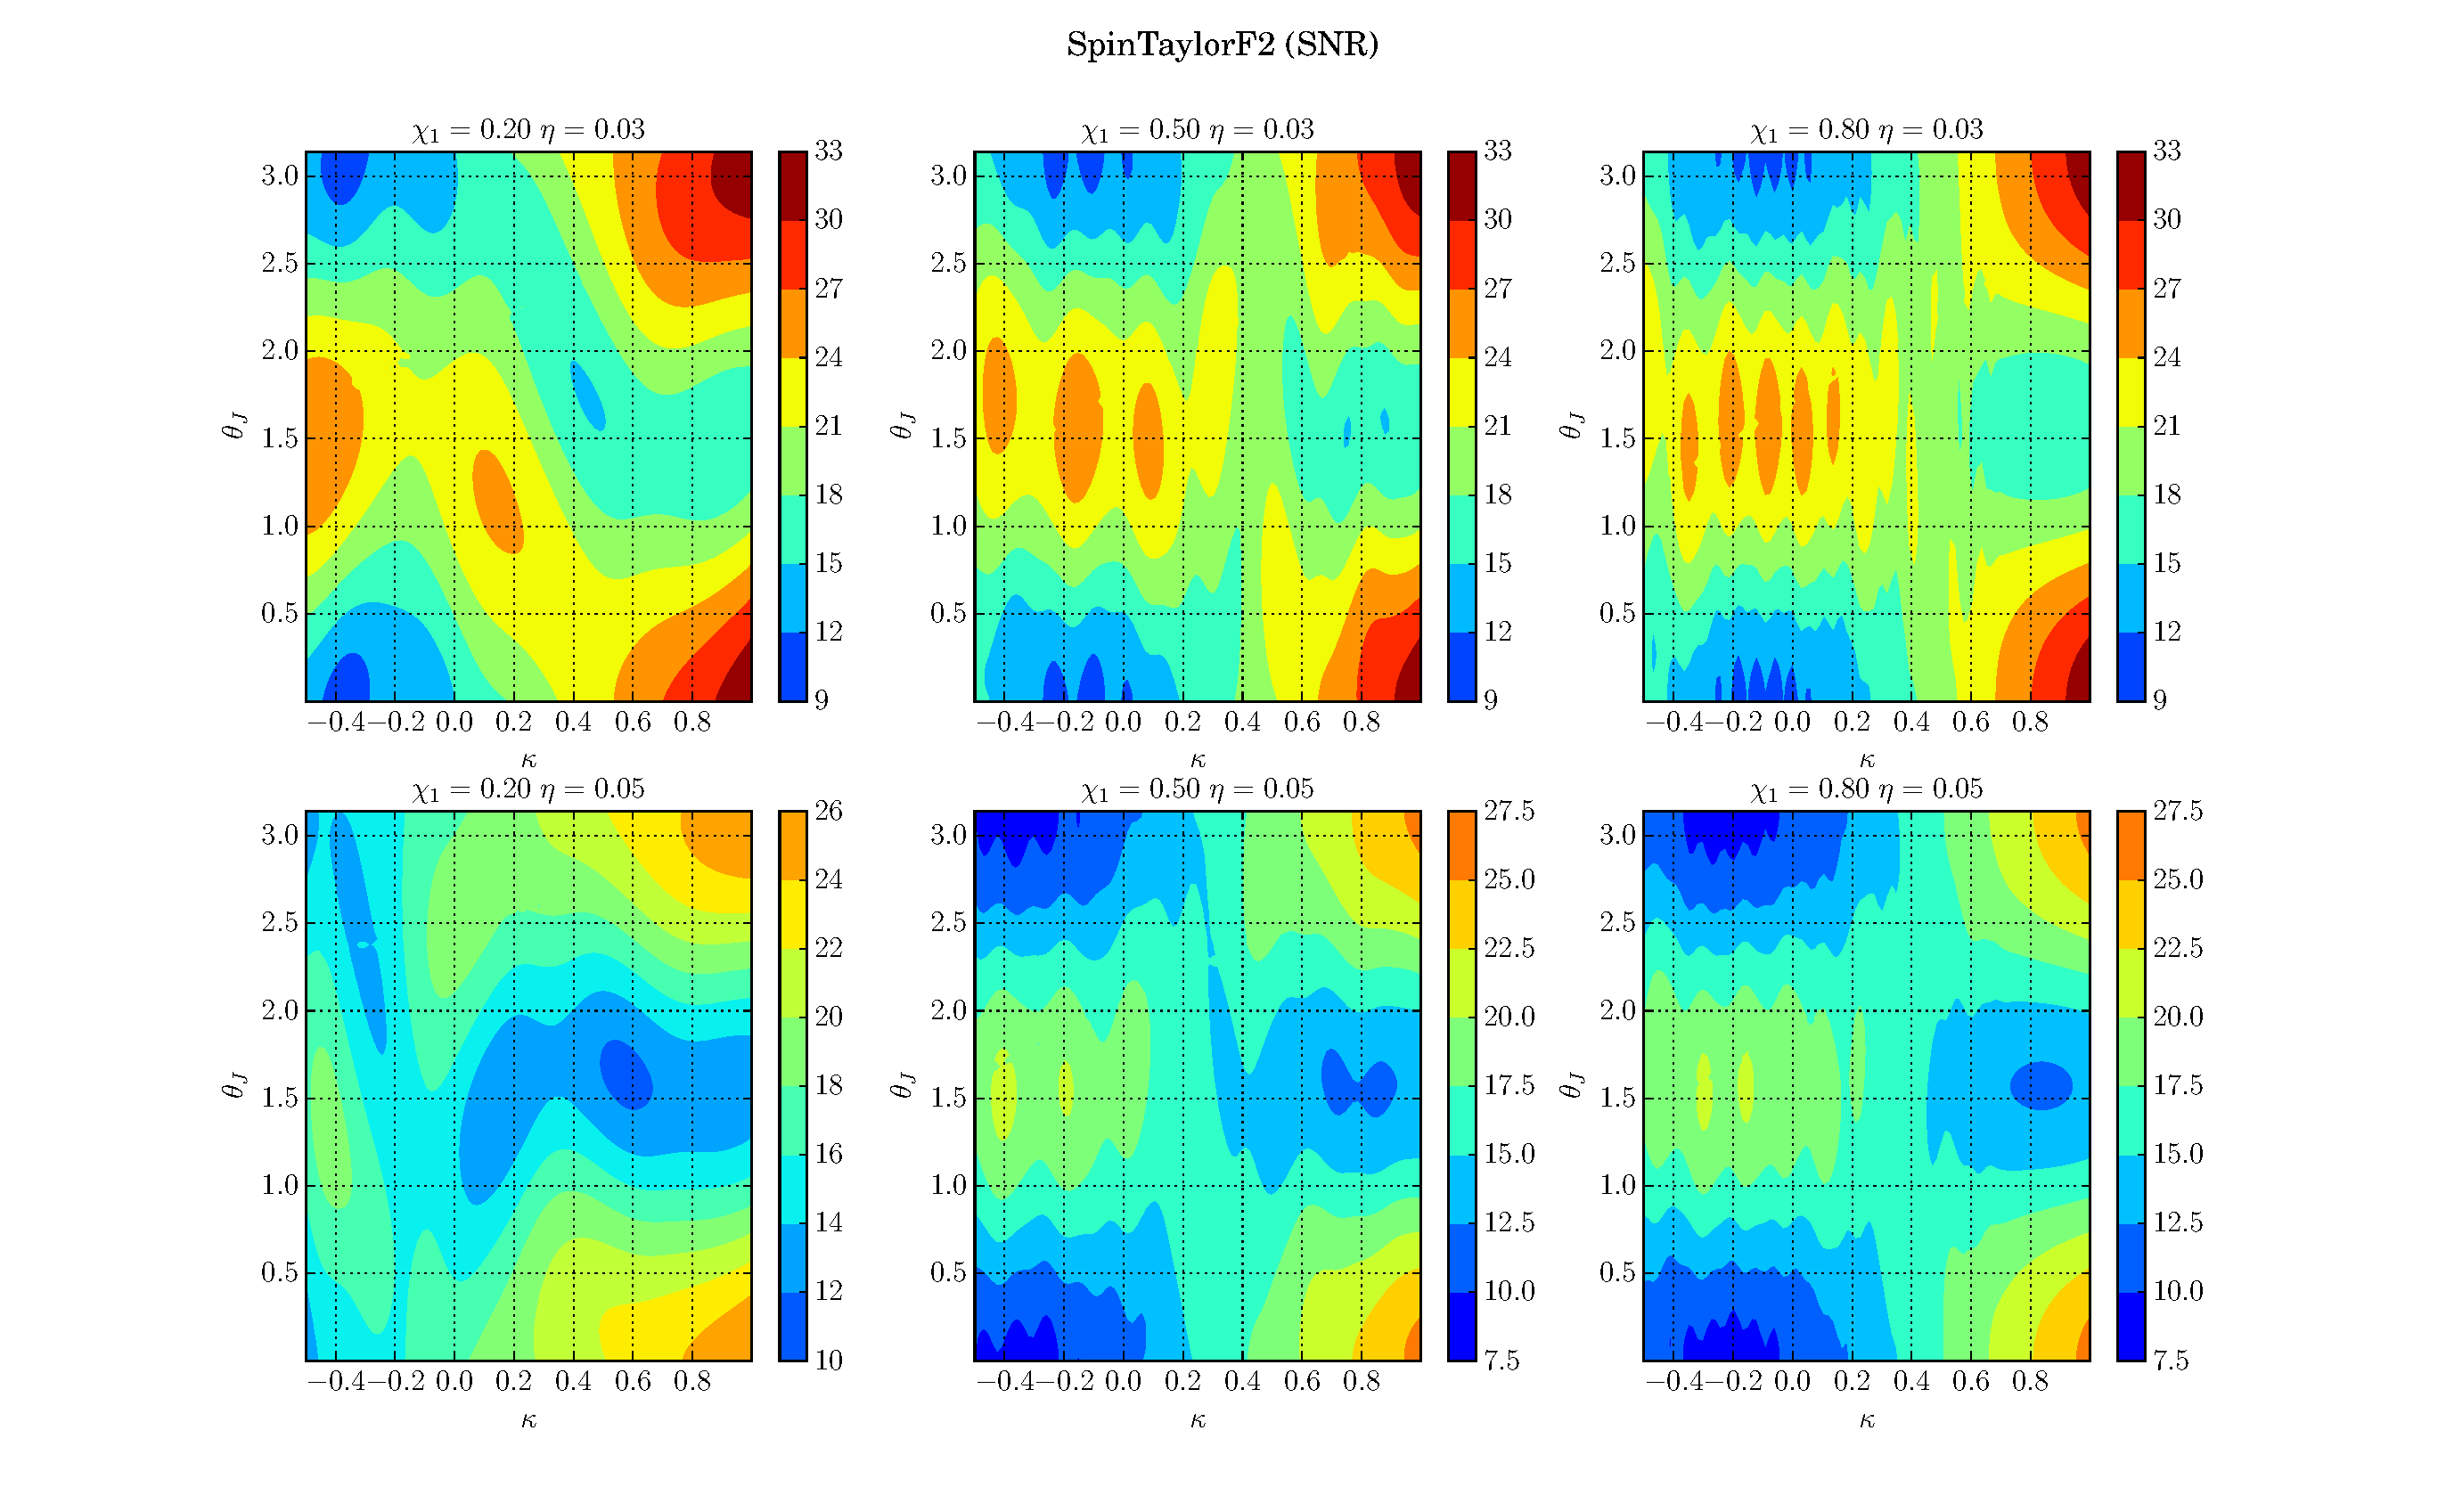
\includegraphics[width=\textwidth]{./images/SNR_GRID_0F.pdf}
\caption{Variation of SNR in the $(\theta_J, \kappa)$ parameter space for 
different $\chi$ and $\eta$ values, where $\chi$ changes over the horizontal 
axis of the grid and $\eta$ varies over the vertical axis of the grid.}
\centering 
\end{figure}

We see that the maximum SNR increases with the increase in black hole mass
(i.e. lower $\eta$). Further, we observe that the SNR is the highest in the
region where  $\theta_{J} = 0$ or $\pi$ which corresponds to the situation where
the the plane of  the binary is directly overhead or underneath us, and for
$\kappa = 1$ which means that  $\mathbf{S}$ is along the direction of
$\mathbf{L}$. Both these features can be explained by simply comparing the
results with expression for the frequency independent part of waveform amplitude 
in the presence of precession (see Eq.~(A4) in~\cite{Apostolatos1994}):
\label{amplitudes}
\begin{equation}
H_{+} = \frac{1}{2}\frac{4 m_{1}m_{2}}{rD} \left[1 + (\hat{\mathbf{L}}\cdot\hat{\mathbf{N}})^{2}\right], 
H_{\times} = \frac{4 m_{1}m_{2}}{rD}\left[\hat{\mathbf{L}}\cdot\hat{\mathbf{N}}\right].
\end{equation}
The above equation suggests that the SNR --- which is directly proportional to
the square of the  amplitude of the waveform -- increases with increasing mass,
and also the fact the amplitudes  are maximum when $\mathbf{L}$ is along the
line of sight $\hat{\mathbf{L}}$. The second condition is precisely what the
combination of $(\theta_J, \kappa)$ satisfies, in regions where the SNR peaks.
The fact that the SNR also peaks near $\theta_J = \pi/2$ for lower values of
$\kappa$, can aslo be explained using Eq.~(\ref{amplitudes}); the argument
however, is more involved.

\section{Overlap study in the $(\theta_J, \kappa)$ parameter space}
We computed the overlaps for all the sidebands $m=-2$
to $m=2$ and observed that the $m=0$ and  $m=2$ sidebands are the dominant
contributors to the total SNR of the full SpinTaylorF2 waveform. In addition, we
found  that the sidebands $m=2$ and $m=0$ dominate in roughly complimentary
regions of the  $(\theta_J, \kappa)$ parameter space --- if the system is highly
precessing, most of the SNR is captured by the $m=0$ sideband, whereas if the
system is mildly precessing the $m=2$ has the dominant contribution to the SNR of
the signal. See Fig.~(\ref{fig:P2}), which shows overlap  of the sidebands $m=2$
and $m=0$ with the full SpinTaylorF2 waveform: regions of high overlap
correspond to regions where the fractional contribution  to the total SNR would
be high. Therefore, the ratio of the SNR's of the two sidebands i.e.
$\text{SNR}_{20}/\text{SNR}_{22}$ can be used as a diagnostic to quantify the
extent of precession in the system. Most importantly, the overlap plots indicate
that the $m=2$ and $m=0$ sidebands can be used for parameter estimation in
appropriate regions of parameter space (i.e regions with high overlap), instead
of the full SpinTaylorF2 waveform, which has the potential to lead a massive reduction in
computational cost associated with waveform generation. 

\label{fig:P2}  \begin{figure}[t]
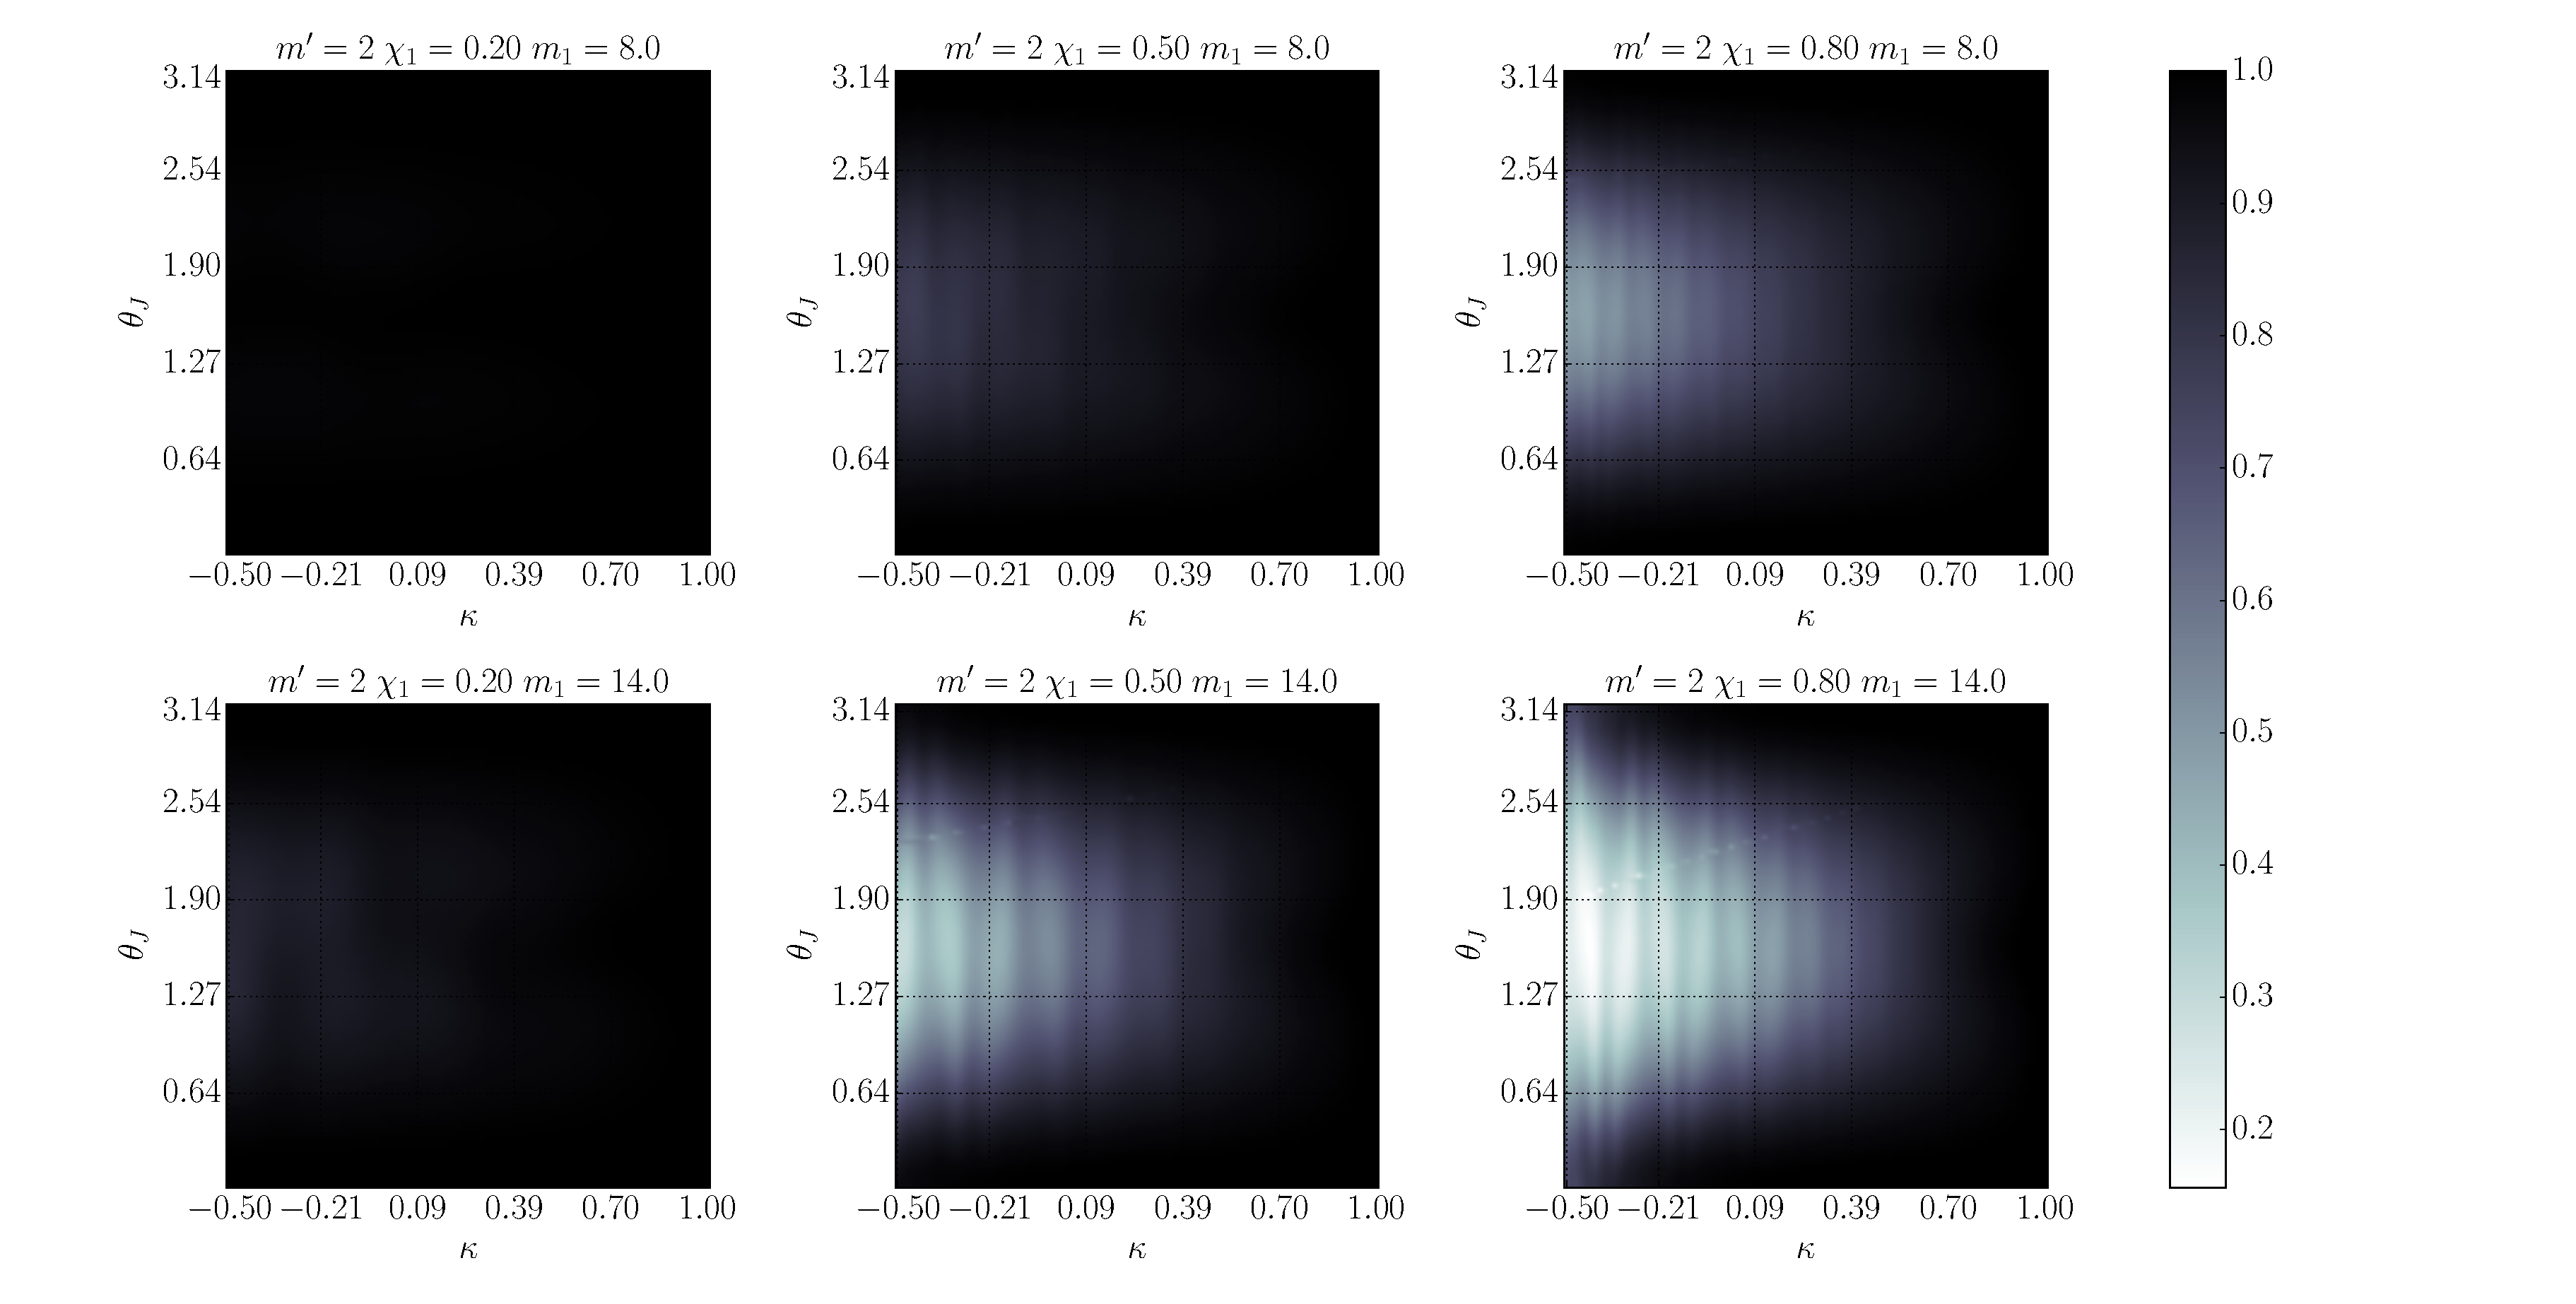
\includegraphics[width=\textwidth]{./images/OVLP_GRID_P2.pdf}
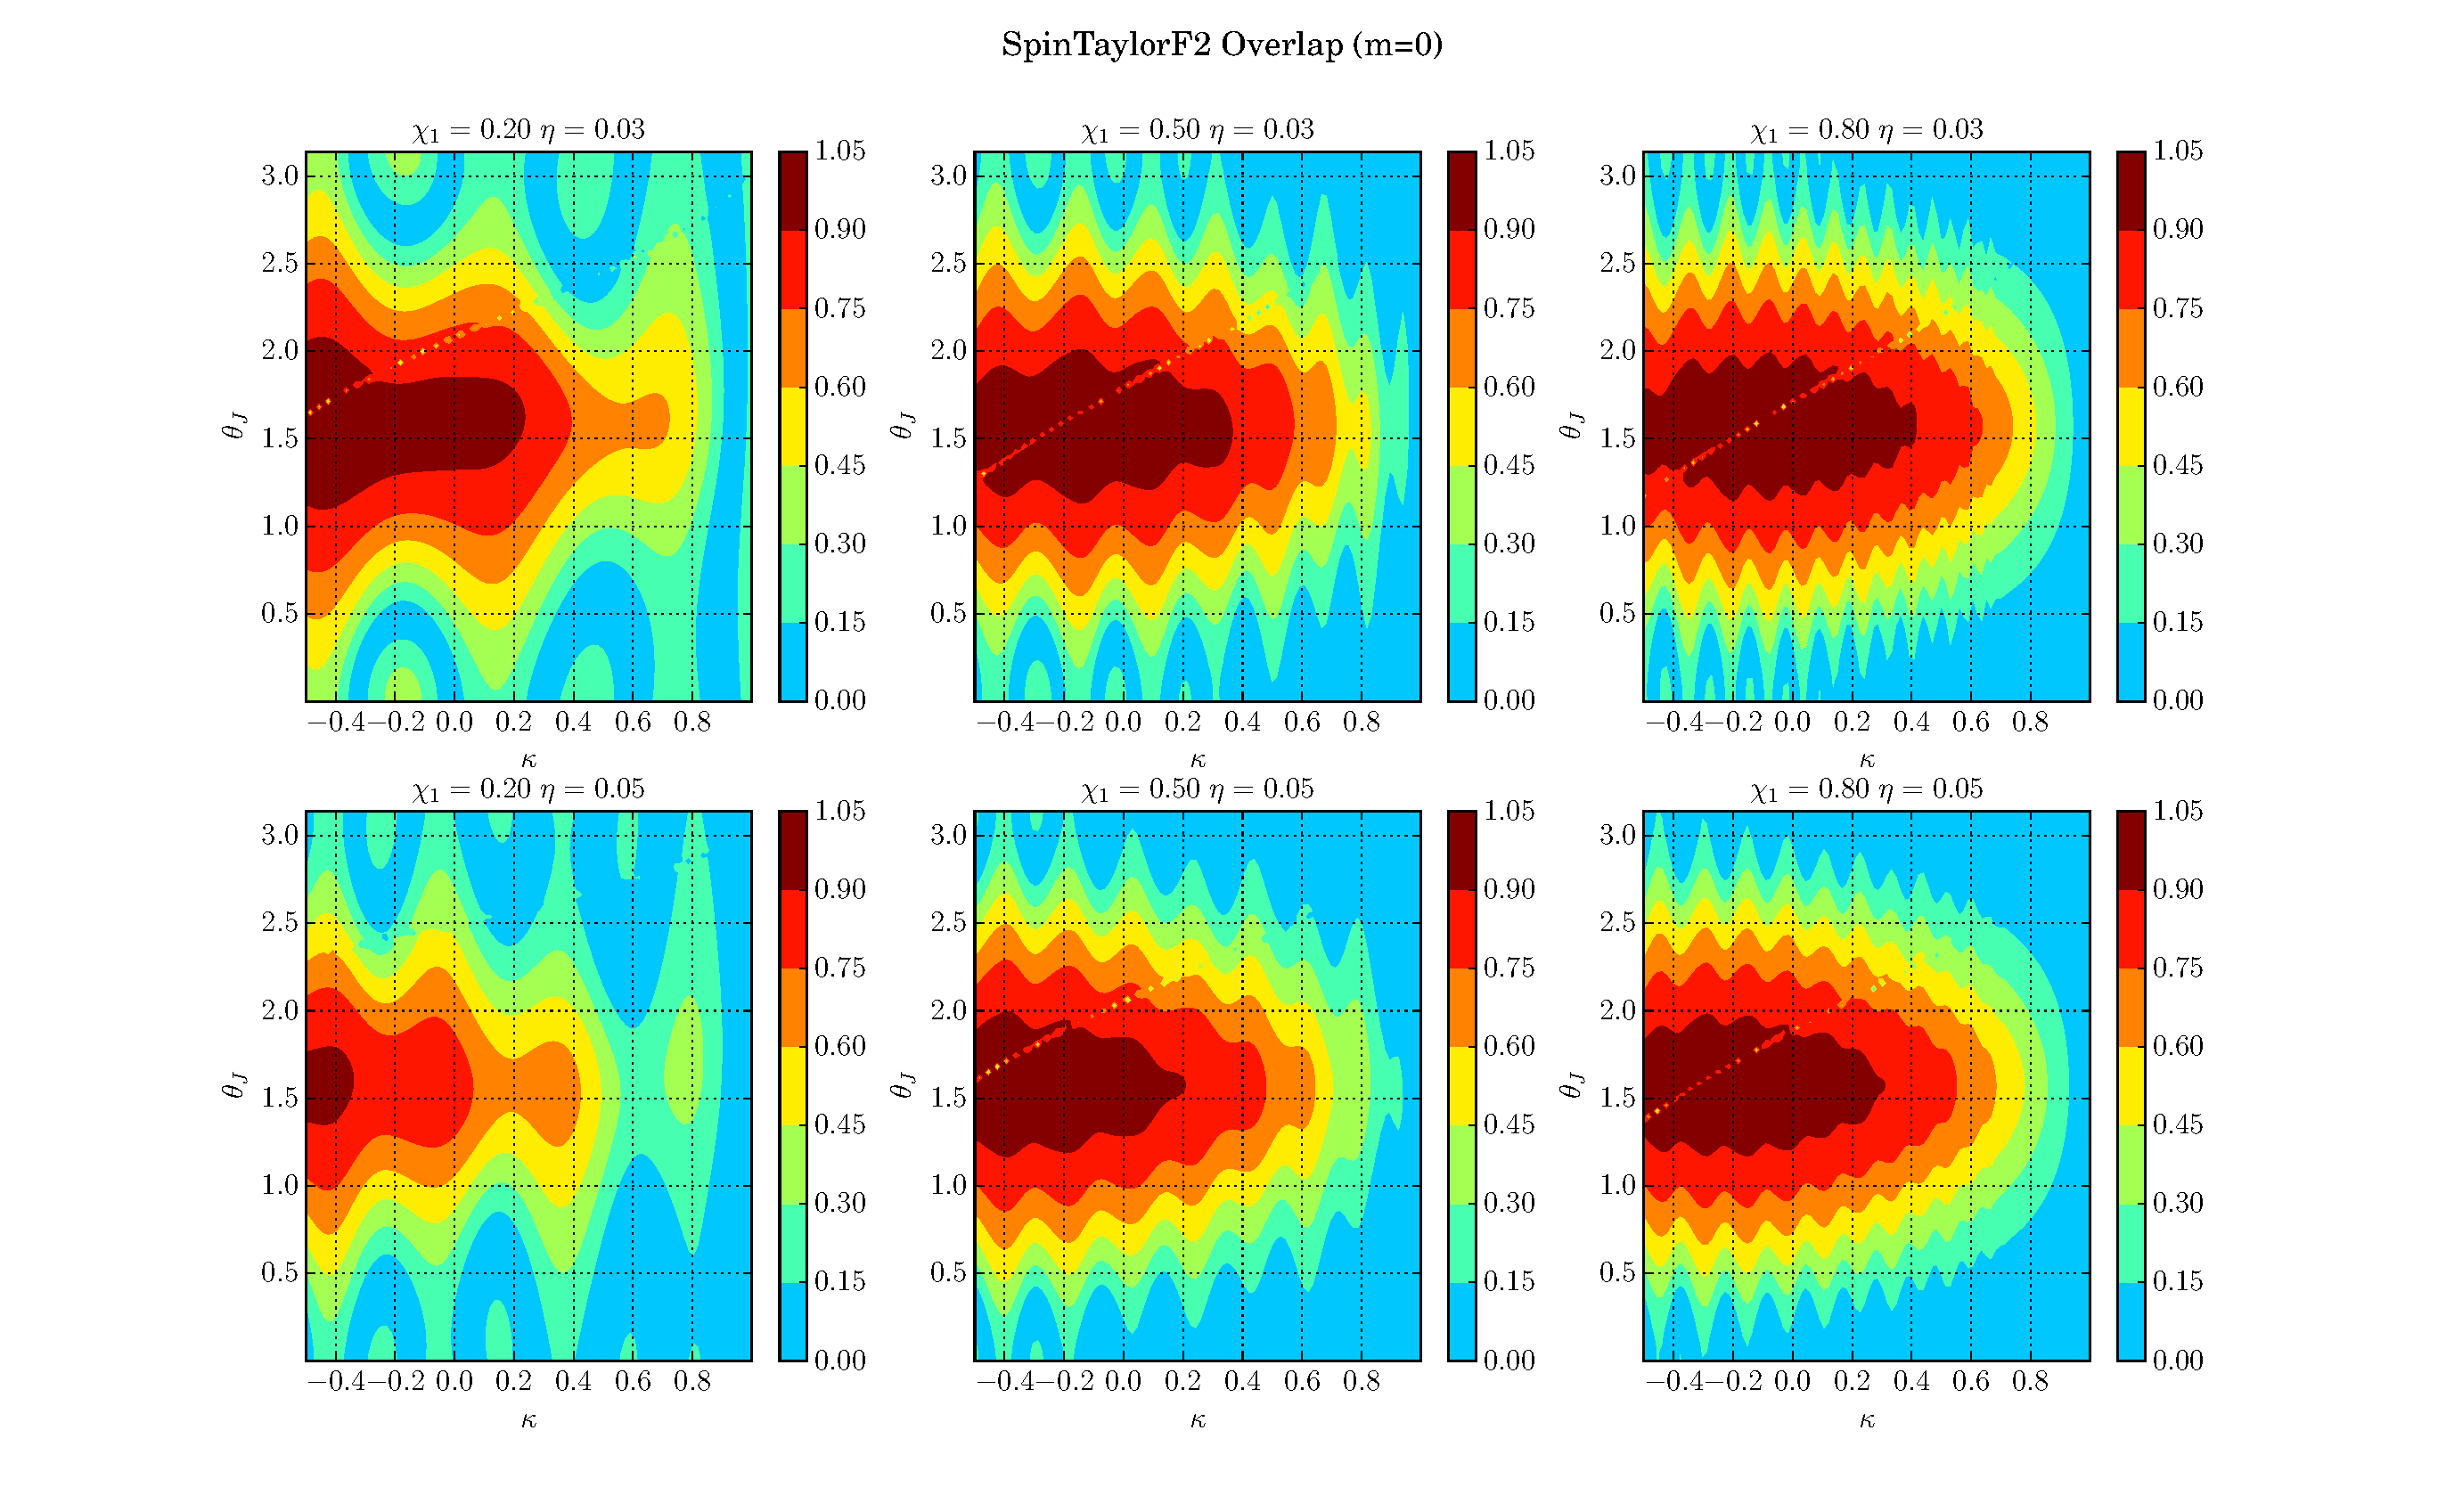
\includegraphics[width=\textwidth]{./images/OVLP_GRID_P0.pdf} \caption{Variation
of overlap of $m=2$ and $m=0$ sideband with the SpinTaylorF2
waveform in the $(\theta_J, \kappa)$ parameter space for  different $\chi$ and
$\eta$ values, where $\chi$ changes over the horizontal  axis of the grid and
$\eta$ varies over the vertical axis of the grid.}  
\centering  
\end{figure}
